\section{Profiler} \label{sec:profiler}
This section describes the use of a profiler to identify bottlenecks in the LUA software. The profiler is used to identify functions that consume a lot of CPU time, and thus are candidates for optimization.

Microsoft Visual Studio (VS) comes with an installation of VSDiagnostics; a command-line profiling tool \cite{vsdiagnostics}. VSDiagnostics generates *.diagsession files, which VS interprets and visualizes. For this reason, it is more convenient to call VSDiagnostics indirectly from within Visual Studio.

To do this, debug and symbol flags need to be added to the compilation commands of object files and final linking of the main executable. Adding these flags ensures the compiler generates symbol (for Windows .pdb) files, which are required by any profiler.

The VS profiler discerns between two categories of CPU time: self-time and total time. Self-time is the time spent in a function, excluding time spent in subroutines/-functions. Total time is the time spent in a function, including time spent in subroutines/-functions \cite{cpu_usage}. The self time is expressed as
\begin{equation}
    \text{self-time} = \frac{\text{CPU time spent in the function}}{\text{total execution time}} \times 100\%.
    \label{eq:self_time}
\end{equation}

\subsection{Profiling test setup}
Profiling measurements are done in a controlled environment, where the LUA software is run with one laser line scanner. The scanner is placed in front of a test setup consisting of a lone ILUC ring, a mockup for the ILUC ribs and new joint.

\begin{figure}[H]
    \begin{subfigure}{0.45\textwidth}
        \centering
        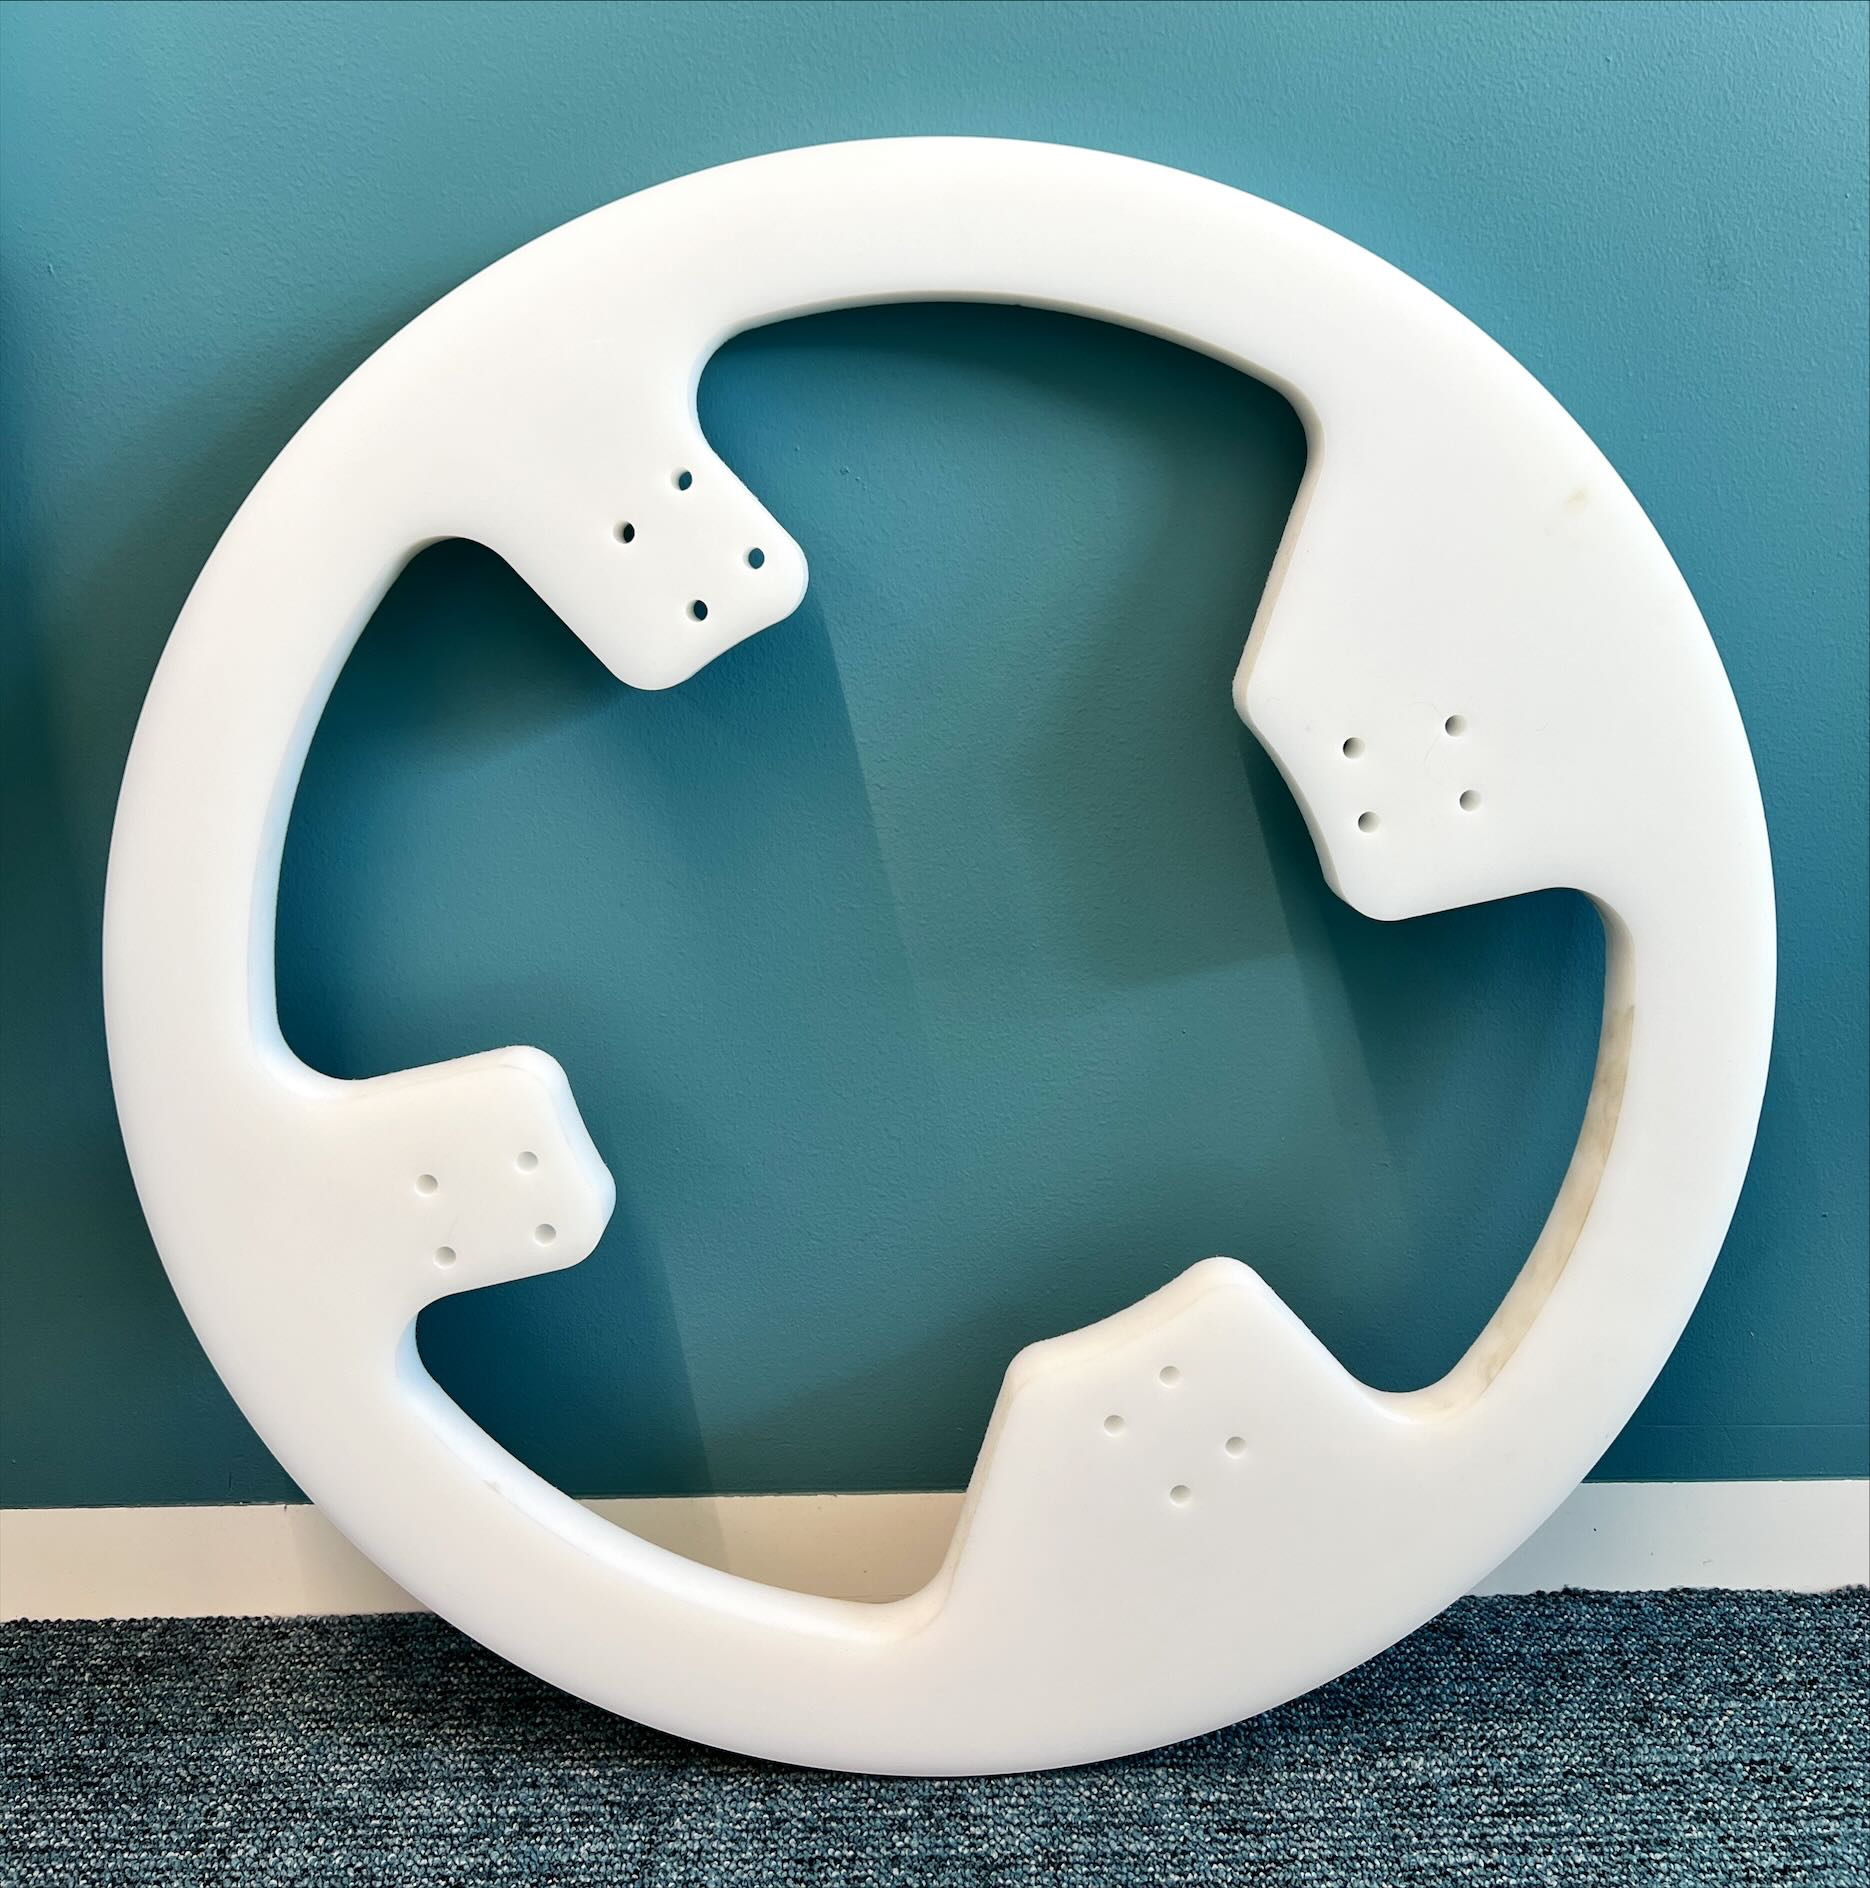
\includegraphics[width=\textwidth]{images/ILUC_ring.jpeg}
        \caption{ILUC ring.}
    \end{subfigure}
    \begin{subfigure}{0.45\textwidth}
        \centering
        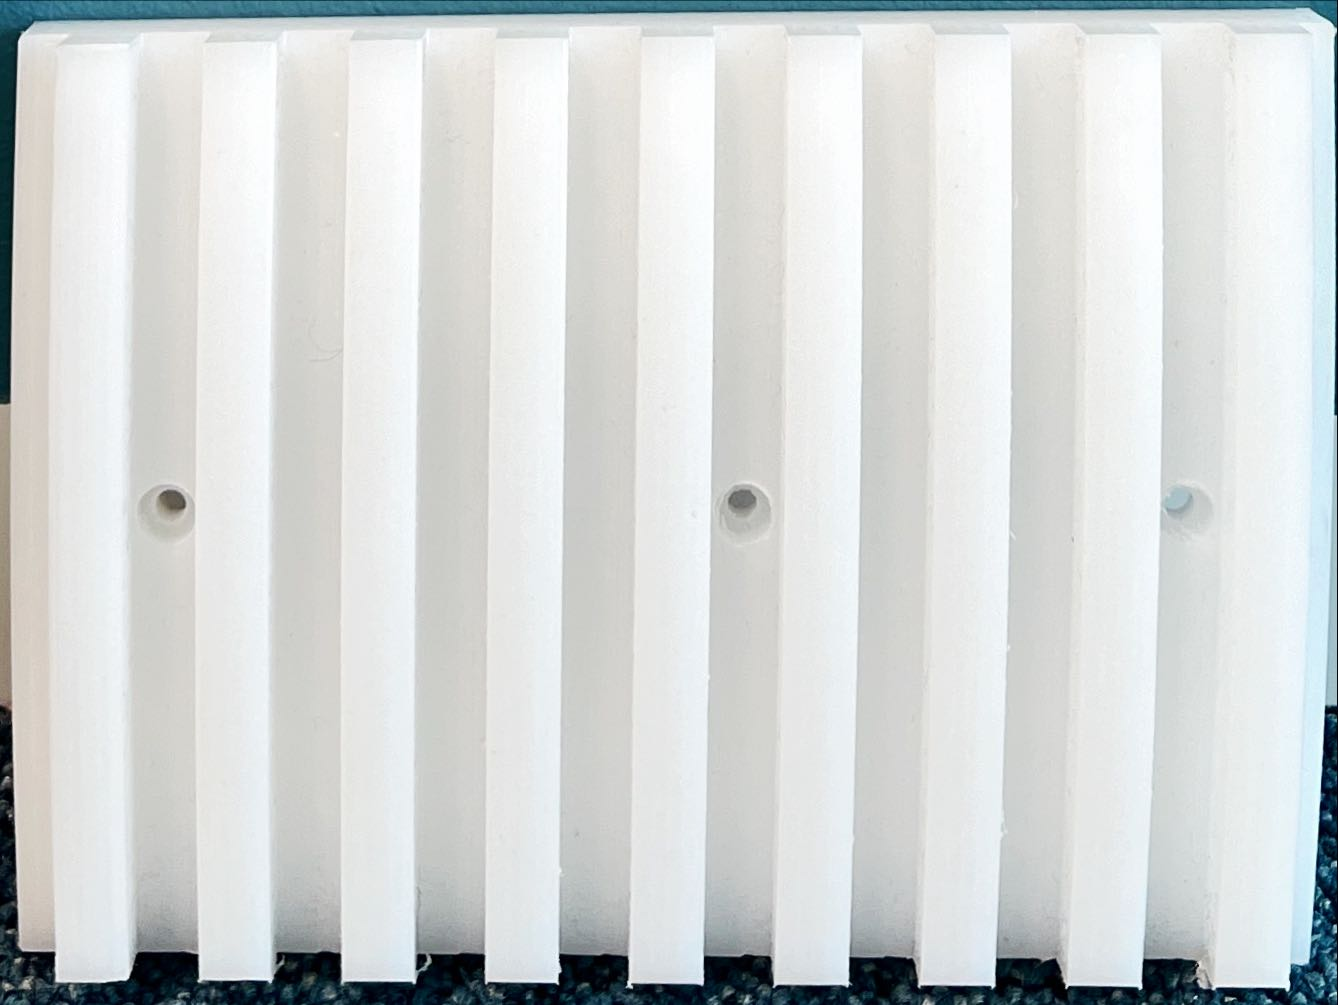
\includegraphics[width=\textwidth]{images/ILUC_ribs_mockup.jpeg}
        \caption{ILUC ribs.}
    \end{subfigure}
    \centering
    \begin{subfigure}{0.9\textwidth}
        \centering
        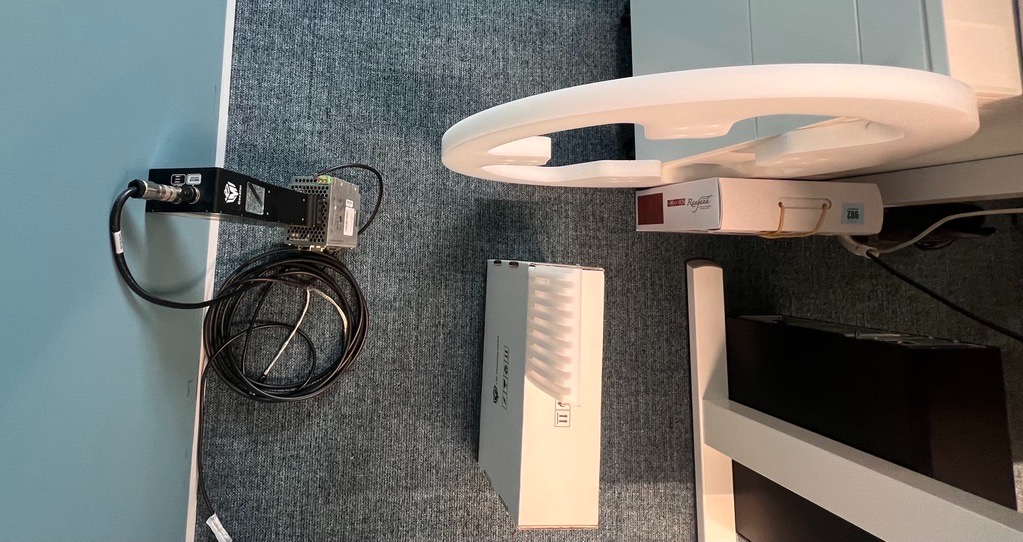
\includegraphics[width=\textwidth]{images/test_setup.png}
        \caption{Full setup. Note, laser is not connected}
    \end{subfigure}
    \caption{The experimental setup for profiling measurements.}
\end{figure}


These objects are moved in a controlled manner to simulate the phased of LUA. The experimental setup is described in Table \ref{tab:experimental_phases}.

\begin{table}[H]
    \centering
    \begin{tabular}{|p{4cm}|p{5.5cm}|p{5cm}|}
        \hline
        \textbf{Phase}& \textbf{Description} & \textbf{Experimental Setup} \\ \hline

        \textbf{\ref{fig:oop_track} Joint recognition} & LUA software detects joint as it moves towards mainline. U-Frame moves with joint after (successful) detection. & Flat surface resembling the joint (back of the ILUC-ribs mockup) is quickly brought into frame and subsequently kept still.\\ \hline

        \textbf{\ref{fig:oop_ILUC_ring} ILUC ring recognition} & Joint and U-Frame move until ILUC ring is detected, after which partial line up takes place. & Next to the joint mockup, the side of the ILUC ring is brought into frame representing the ILUC-ring.\\ \hline

        \textbf{\ref{fig:oop_ILUC_ribs} ILUC ribs recognition} & The ILUC-ring moves into the joint during the aforementioned partial line-up, after which the ILUC-ribs are detected. The joint is moved over the ribs towards the mainline. & A joint mockup (a side of the ILUC-ring mockup) is still in frame. The ILUC ribs mockup is slowly moved into frame, revealing all its ribs. \\ \hline

        \textbf{\ref{fig:oop_final_line_up} Final line up}  & The mainline gets detected and the joint is lined up with & The joint mockup and a second flat surface (mainline mockup) are slowly moved together. \\ \hline
    \end{tabular}
    \caption{Profiling experiments simulating essentials phases of LUA. Each of the experiments are performed with one laser line scanner and done on a standard company PC (HP Z4 G4).}
    \label{tab:experimental_phases}
\end{table}

Every profiling test is approximately 20 seconds in length, in keeping with the profiling guidelines. Every test is preceded by a 20 second settling period during which the LUA software runs, but no profiling or setup movement takes place. The profiling sampling rate is >=1000 Hz.

\subsection{Profiling results} \label{ssec:profiling_results}
Shown in Table \ref{tab:profiling_results} are the most time consuming functions per LUA phase.

\begin{table}[H]
    \centering
    \begin{tabular}{|p{4cm}|p{7cm}|p{2.5cm}|}
        \hline
        \textbf{Phase}                 & \textbf{Top function}                                          & \textbf{self-time (\%)} \\ \hline
        \textbf{Joint recognition}     & \lstinline[language=c]|LineFinder::calculateNrPointsInEachBin| & 13.94                   \\ \hline
        \textbf{ILUC ring recognition} & \lstinline[language=c]|LineFinder::calculateNrPointsInEachBin| & 17.89                   \\ \hline
        \textbf{ILUC ribs recognition} & \lstinline[language=c]|LineFinder::calculateNrPointsInEachBin| & 18.53                   \\ \hline
        \textbf{Final line up}         & \lstinline[language=c]|LineFinder::calculateNrPointsInEachBin| & 15.87                   \\ \hline
    \end{tabular}
    \caption{Profiling results.}
    \label{tab:profiling_results}
\end{table}

The results show that the function \lstinline[language=c]|LineFinder::calculateNrPointsInEachBin| is the most time consuming function in all phases. This function is a bottleneck and is a target for optimization.

As mentioned in section \ref{ssec:code_flow}, recognition of the ILUC ribs is the most time consuming phase. This can be attributed to the ILUC ribs consisting of many smaller line segments. The Hough transform function executed in each of the profile analyser threads in figure
\ref{fig:code_flow} is ran for each of these line segments. This in turn results in many calls to the function \lstinline[language=c]|LineFinder::calculateNrPointsInEachBin|, which is a part of the Hough transform.

Figure \ref{fig:profiling_bottleneck} shows profiling results of parts of the bottleneck function
\begin{figure}[H]
    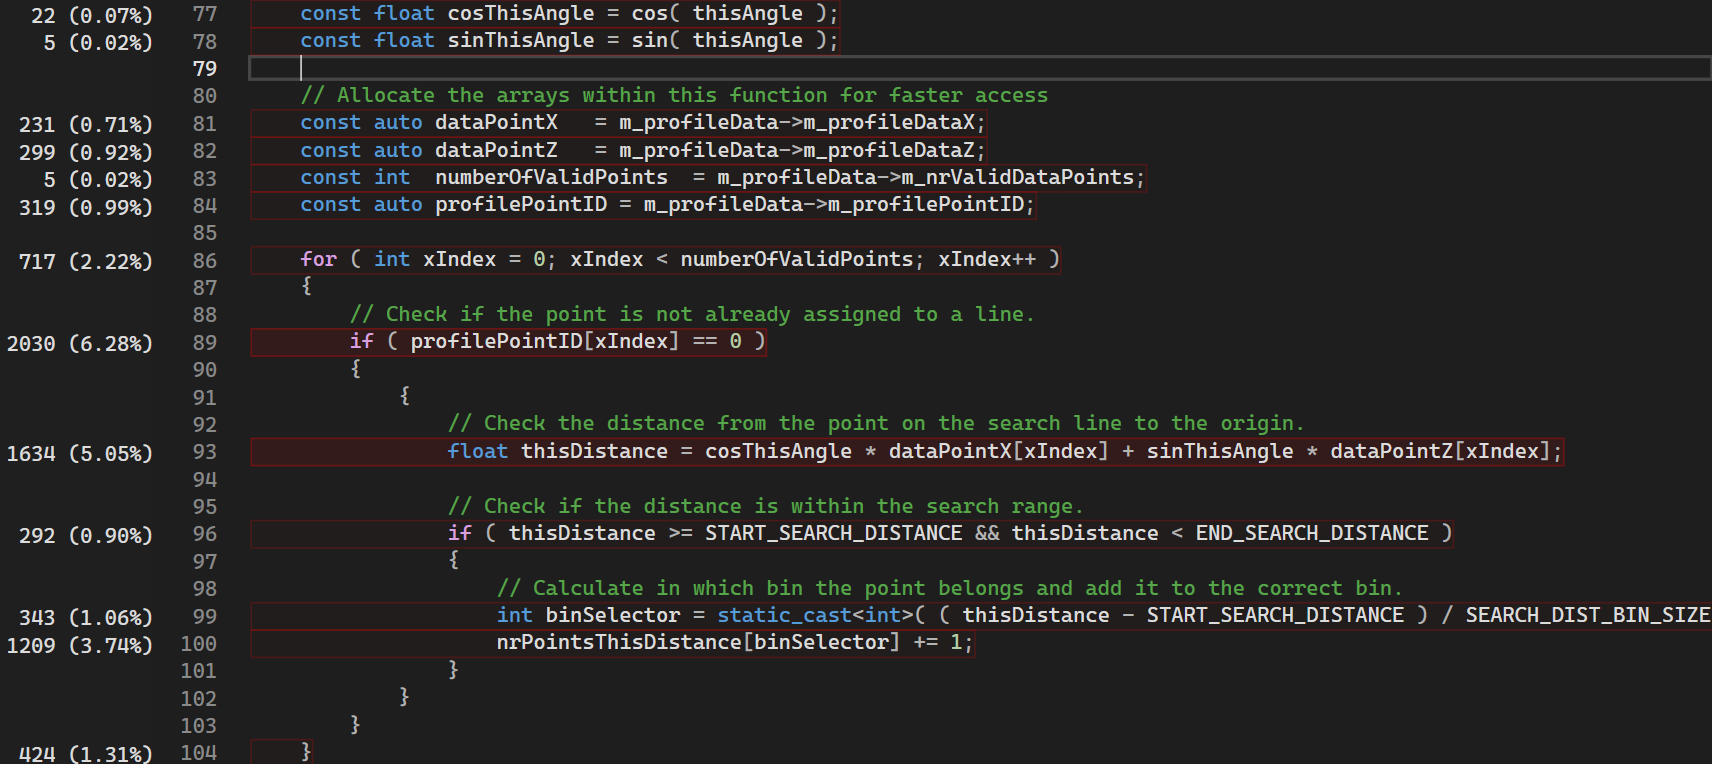
\includegraphics[width=\textwidth]{images/profiling_bottleneck.png}
    \caption{Profiling results of the function \lstinline[language=c]|LineFinder::calculateNrPointsInEachBin| during the ILUC ribs recognition phase.}
    \label{fig:profiling_bottleneck}
\end{figure}

From figure \ref{fig:profiling_bottleneck} it becomes clear what the most time consuming operations are in the calculation of the Hough transform. In order of most time consuming to least, these are:
\begin{enumerate}
    \item Checking if a data point is not already associated to a line (\textbf{line 89 in figure \ref{fig:profiling_bottleneck}});
    \item Calculating the distance between a data point the laser line scanner's origin (\textbf{line 93 in figure \ref{fig:profiling_bottleneck}});
    \item  Determining in which distance bin a data point falls (\textbf{line 100 in figure \ref{fig:profiling_bottleneck}}).
\end{enumerate}